El presente informe detalla el análisis a la implementación
de una multiplicación de matrices de forma paralela en GPU~\footnote{
Capítulo 6 - \url{http://developer.download.nvidia.com/compute/cuda/1_1/NVIDIA_CUDA_Programming_Guide_1.1.pdf} 
}.

La idea principal de la implementación y paralelización,
es poder dividir las matrices en pequeños rectángulos,
es decir, seleccionar bloques, y dentro de cada uno de esos bloques,
las hebras serán las responsables de realizar la multiplicación
de los elementos en su interior.

Para este caso se ha considerado una multiplicación de matrices
cuadradas, aunque la función sigue siendo válida para matrices
no cuadradas.

El procedimiento de la multiplicación es sencillo,
primero se cargan las dos matrices de la memoria global a la memoria compartida,
cada hebra carga un elemento y guarda resultado de multiplicación,
luego se escriben en la memoria global una vez terminanados todos.

Una de las fortalezas es el buen uso de la memoria compartida,
donde se mejora el ancho de banda del acceso a la memoria global,
ya que sólo se leen A y B $n$ veces, donde $n$ es el tamaño del ancho de la matriz
A dividio por el tamaño del bloque (width A / block size).

En la documentación se señala también,
que no es la implementación más óptima para éste problema,
que sólo se trata de representar varios principios y mecanismos
de la programación en GPU.

\subsection{Implementación}

Consta de una función en el \texttt{device},
una función en el \texttt{host} y el \texttt{main}.

La idea es obtener la matriz C, de la multiplicación de las matrices A y B:
$$C\ =\ A\ \cdot\ B$$

\begin{itemize}
	\item \texttt{main()}
	\begin{itemize}
		\item Asignar memoria a C.
		\item Leer archivo con datos y crear matrices.
		\item Llamar a \texttt{Mul()}
	\end{itemize}
	\item \texttt{Mul()} (host)
	\begin{itemize}
		\item Cargar las matrices A y B, copiando sus valores.
		\item Cargar la matriz vacia C en el device.
		\item Calcular la dimensión del Bloque y del Grid.
		\item Llamada al kernel \texttt{Muld()}
		\item Leer C del device.
	\end{itemize}
	\item \texttt{Muld()} (device)
	\begin{itemize}
		\item Calcular índices, para deteriminar la posición de inicio y fin de submatrices,
		sin dejar de lado el tamaño del paso por cada iteración.
		\item Loop de cálculo:
		 \begin{itemize}
		 	\item Memoria compartida para las submatrices.
			\item Cargar sub-matrices de memoria global a memoria compartida.
			\item Multiplicar sub-matrices.
		 \end{itemize}
		\item Escribir las sub-matrices a la memoria global.
	\end{itemize}
\end{itemize}

\section{Pruebas}

Las pruebas se realizaron con 2 matrices de dimensiones,
$1600x1600$, generando $2560000$ números aleatorios
para cada matriz.

Se realizó una implementación para comparar,
sin utilizar programación paralela en C++.

\begin{table}[!ht]
\begin{center}
	\begin{tabular}{|l|c|c|c|c|c|c|c|c|c|c|}
		\hline
		\texttt{BLOCK\_SIZE} & 2 & 4 & 5 & 8 & 10 & 16 & 20 & 25 & 32 & 40 \\\hline
		\texttt{Tiempo [s]}  & 44.009 & 9.27 & 6.521 & 5.139 & 5.991 & 4.659 & 4.499 & 1.986 & 2.002 & 2.087 \\\hline
	\end{tabular}
	\\
	\begin{tabular}{cc}
		Tiempo en CPU: & 52.881 [s] \\
	\end{tabular}
\end{center}
\caption{Tabla de resultados}
\label{table:1}
\end{table}

\begin{figure}
\begin{center}
	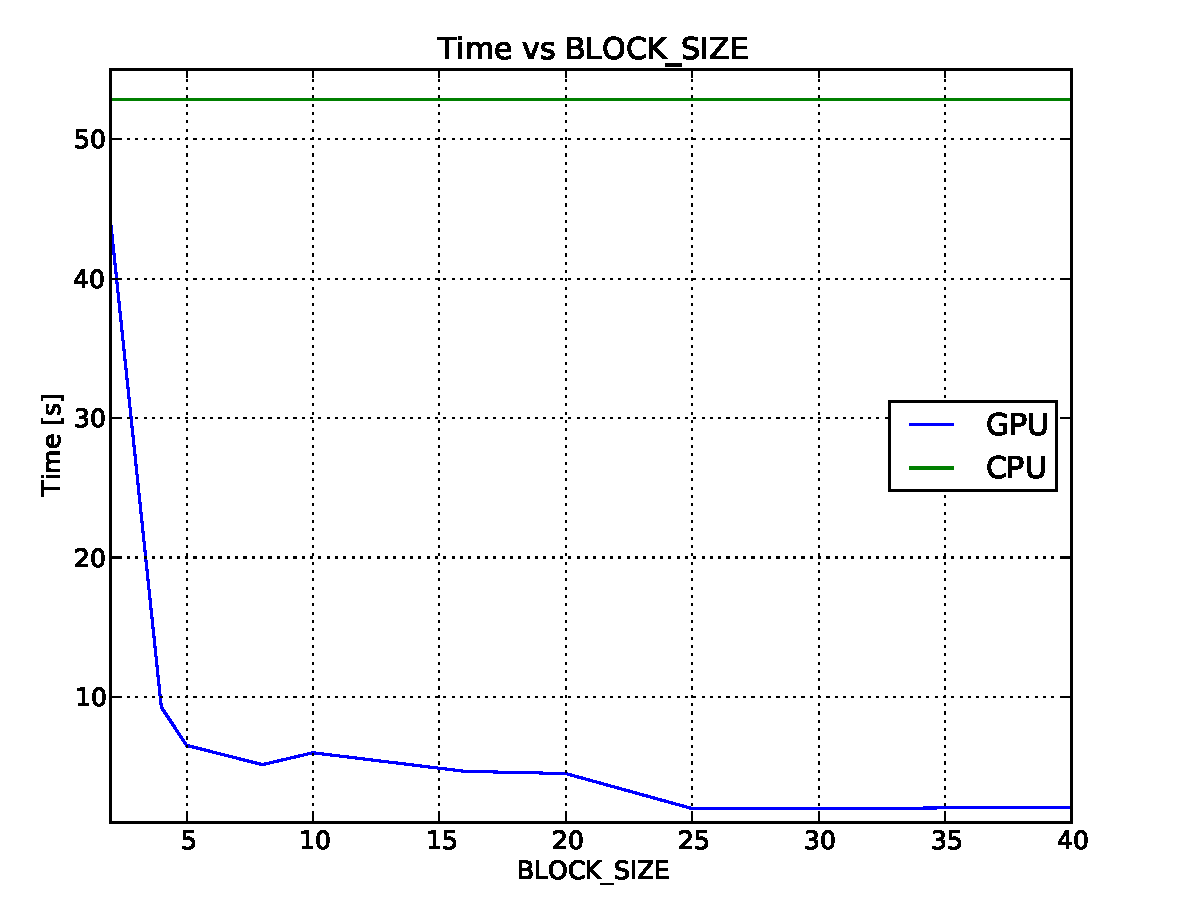
\includegraphics[width=0.5\textwidth]{img/plot-proyecto.pdf}
\end{center}
\caption{Resultados entre el \texttt{BLOCK\_SIZE} y el Tiempo}
\label{fig:1}
\end{figure}

Los experimentos fueron realizados con distintos tamaños de
valores para el \texttt{BLOCK\_SIZE} (ver tabla ~\ref{table:1}), cuidando de que fueran
múltiplos de el ancho de las matrices.

Los valores no sobrepasaron a $40$ debido a que con números
mayores, la compilación fallaba por utilizar muchos datos compartidos.

Podemos ver en la figura~\ref{fig:1} que con \texttt{BLOCK\_SIZE} pequeño como es 2,
el resultado no sirve casi de nada, por el sentido de que sería practicamente hacer
la misma multiplicación por cada elemento, sin ocupar paralelismo,
en cambio luego que vamos aumentando el tamaño del bloque,
notamos el aumento del desempeño de la implementación, llegando
a 25 como un óptimo para éste ejemplo, puesto que despues se comporta
muy similar.

Como era de esperarse, la CPU perdió frente a la GPU,
debido a que no está paralelizado y sólo funciona en un procesador
normal.

Por otro lado, debido a que el ancho de cada matriz A y B
son múltiplos siempre del \texttt{BLOCK\_SIZE}, el
\emph{global memory coalescing} está asegurado.

Tampoco hay un conflicto \emph{Shared Memory Bank}, por que los índices
de las hebras son los mismo y van variando de 0 a \texttt{(BLOCK\_SIZE-1)},
entonces las hebras van accediendo a distintos espacios de memoria.

La implementación cuida bien de no sufrir algún problema de \emph{divergencia},
pudiendo sincronizar las hebras en las 2 ocaciones más importantes
del cálculo, cuando se cargan las matrices de la memoria global a compartida,
y luego de que se calculo la sub-matriz C en cada iteración.
